% THIS IS SIGPROC-SP.TEX - VERSION 3.1
% WORKS WITH V3.2SP OF ACM_PROC_ARTICLE-SP.CLS
% APRIL 2009
%
% It is an example file showing how to use the 'acm_proc_article-sp.cls' V3.2SP
% LaTeX2e document class file for Conference Proceedings submissions.
% ----------------------------------------------------------------------------------------------------------------
% This .tex file (and associated .cls V3.2SP) *DOES NOT* produce:
%       1) The Permission Statement
%       2) The Conference (location) Info information
%       3) The Copyright Line with ACM data
%       4) Page numbering
% ---------------------------------------------------------------------------------------------------------------
% It is an example which *does* use the .bib file (from which the .bbl file
% is produced).
% REMEMBER HOWEVER: After having produced the .bbl file,
% and prior to final submission,
% you need to 'insert'  your .bbl file into your source .tex file so as to provide
% ONE 'self-contained' source file.
%
% Questions regarding SIGS should be sent to
% Adrienne Griscti ---> griscti@acm.org
%
% Questions/suggestions regarding the guidelines, .tex and .cls files, etc. to
% Gerald Murray ---> murray@hq.acm.org
%
% For tracking purposes - this is V3.1SP - APRIL 2009

\documentclass{acm_proc_article-sp}
\usepackage{url}
\begin{document}

\title{Efficient graph-based image segmentation of aerial images for road
detection\titlenote{This report was written in the spring of 2013 in the
advanced level course MAA507 "Mathematics behind internet" at M\"{a}lardalen
University, Sweden. Best viewed in color.}}
%\subtitle{[Extended Abstract]
%\titlenote{A full version of this paper is available as
%\textit{Author's Guide to Preparing ACM SIG Proceedings Using
%\LaTeX$2_\epsilon$\ and BibTeX} at
%\texttt{www.acm.org/eaddress.htm}}}
%
% You need the command \numberofauthors to handle the 'placement
% and alignment' of the authors beneath the title.
%
% For aesthetic reasons, we recommend 'three authors at a time'
% i.e. three 'name/affiliation blocks' be placed beneath the title.
%
% NOTE: You are NOT restricted in how many 'rows' of
% "name/affiliations" may appear. We just ask that you restrict
% the number of 'columns' to three.
%
% Because of the available 'opening page real-estate'
% we ask you to refrain from putting more than six authors
% (two rows with three columns) beneath the article title.
% More than six makes the first-page appear very cluttered indeed.
%
% Use the \alignauthor commands to handle the names
% and affiliations for an 'aesthetic maximum' of six authors.
% Add names, affiliations, addresses for
% the seventh etc. author(s) as the argument for the
% \additionalauthors command.
% These 'additional authors' will be output/set for you
% without further effort on your part as the last section in
% the body of your article BEFORE References or any Appendices.

\numberofauthors{1} 
% I've updated the number of authers ~ Christoffer 2012-10-14

%  in this sample file, there are a *total*
% of EIGHT authors. SIX appear on the 'first-page' (for formatting
% reasons) and the remaining two appear in the \additionalauthors section.
%
\author{
% You can go ahead and credit any number of authors here,
% e.g. one 'row of three' or two rows (consisting of one row of three
% and a second row of one, two or three).
%
% The command \alignauthor (no curly braces needed) should
% precede each author name, affiliation/snail-mail address and
% e-mail address. Additionally, tag each line of
% affiliation/address with \affaddr, and tag the
% e-mail address with \email.
%
% 1st. author
\alignauthor
Christoffer Holmstedt\\
       \email{christoffer.holmstedt@gmail.com}
}
% There's nothing stopping you putting the seventh, eighth, etc.
% author on the opening page (as the 'third row') but we ask,
% for aesthetic reasons that you place these 'additional authors'
% in the \additional authors block, viz.
% \additionalauthors{Additional authors: John Smith (The Th{\o}rv{\"a}ld Group,
%email: {\texttt{jsmith@affiliation.org}}) and Julius P.~Kumquat
%(The Kumquat Consortium, email: {\texttt{jpkumquat@consortium.net}}).}
%\date{30 July 1999}
% Just remember to make sure that the TOTAL number of authors
% is the number that will appear on the first page PLUS the
% number that will appear in the \additionalauthors section.

\maketitle
\begin{abstract}
This report goes through the Efficient Graph-Based Image Segmentation algorithm
and its usefulness on aerial images for road recognition with the purpose of
automating the process to create maps. Written as a part of an advanced level course
this report will give the reader an introduction to some basics of digital
image processing, the algorithm and how it all comes together in the application
of aerial images. The report concludes that without additional preprocessing or more
advanced definition of the threshold function the algorithm is of no use
in this application.
\end{abstract}

% A category with the (minimum) three required fields
\category{A.1}{General Literature}{Introductory and Survery}
%A category including the fourth, optional field follows...
% If we want to add another category (or several).
%\category{D.2.8}{CHANGE THIS Software Engineering}{Metrics}[complexity measures, performance measures]

\terms{Theory}

\keywords{Graph-theoretic methods, Object recognition} % NOT required for Proceedings

\newpage
\section{Introduction}
OpenStreetMap is a map built by its users. Users go out to track roads and
other objects with GPS positioning and then adds that information together with
interesting metadata to the OpenStreetMap project. This information is then
available for all its users under a free and open license. The process of
gathering GPS positions for all objects in the world is quite time consuming
so instead of tracking objects by foot some aerial imagery sources are
available so users can stay at home and add objects to the project with the
aerial imagery as source.

Even to add objects manually from aerial images can sometimes be cumbersome and
tedious. This process can be automated and let the user approve with or
without small modications the end result. This would free up time for the
users to spend on other mapping activities such as adding house numbers,
locations of emergency services and other points of interests.

Another purpose to motivate this work is the problem of alignment for
different image sets. The entire world can not fit in a single image
and still include enough detail to see roads, houses and other objects.
Instead stitching is applied where e.g. fixed-wing airplanes fly at a fixed
altitude and in a constant speed and takes several images over a large area.
These images are then "stitched" together to create a large map with enough detail.

In theory this would create a perfect map over a large area though in practice
several problems arise. Some aerial images are photographed at an angle and
creates misalignment cause of this. Other image sets comes with erroneous metadata
such as wrong GPS positions. With GPS traces of roads already added to OpenStreetMap
and automatic road recognition from the aerial imagery it would be possible to
set individual offset for all images to match the positioning of GPS traces.

A third motivating factor is somewhat related to the first problem mentioned above.
When high detail images over areas which have not been mapped before (or old
images are updated with increased detail) are added to sources like Bing maps
it can take sometime before anyone notices the new image. If an automated
process could look through all new images and send notifications to active
users it could increase response time.

% Another usage would be to create a network of roads as node and map that to
% already traced GPS nodes/networks. This would give the possibility to
% automatically align misaligned aerial images for the OpenStreetMap project.

\begin{itemize}
% OpenStreetMap (OSM) is a crowdsourced map built by users collecting gps-traces
%and tracing objects through a few aerial imagery sources that are available.
%...something about JOSM...
%...about this report...
%...The structure of this report...
% In Appendix more thourough look at OpenStreetMap and Java OpenStreetMap Editor
% is given.
% In Appendix "How to use implementation"
% In Appendix "Algorithm recap, with suggested values for application"
%
% Write about 4/8/Mixed choices and how that can affect.
% Define Tau for my use case and explain in the general case.
%
% ...notes while reading medical phd report...
% Goal with this project is a fully automatic process, no human interaction.
    \item Background OSM why use bing maps? What are they used for? if no or only
        a few gps traces exists they can be used to improve the detail of the 
        open street map.
    \item Problems with using Bing maps?
    \item Images are not photgraphed straight above, this gives us different problems.
        \begin{itemize}
            \item Curvy roads
            \item misalignment
            \item
        \end{itemize}
    \item Idea, how to use bing maps, three different questions.
        \begin{itemize}
            \item Automatically calculate bing aerial imagery offset.
            \item
            \item
        \end{itemize}
    \item So alot of problems with Bing maps and image analysis exists
        we are only to look at the image segmentation problem
        and why speed matters in this application.
    \item
    \item
    \item
\end{itemize}


\section{Method}
Method text goes in here.

\section{Digital Image Processing}
Digital image processing is a wide research field with many subspecialities.
Gonzalez and Woods \cite{gonzalez2008} goes in their book through some of them.
From image representation to transformations, filtering, restoriation and finishes
of with compression, segmentation and recognition. To be able to better grasp
the image segmentation algorithm in the following chapters some basics will be
explained first.

\subsection{Digital image representation}
To be able to present, transfer and alter a digital image we first need someway
to represent it on a computer. This is generally done by dividing an image into
its smallest part, {\em pixels}. Each pixel holds a value that defines its {\em intensity}.
The simplest kind of image is a binary-image. Each pixel has a value of either
0 or 1, where 0 means no intensity and 1 means maximum intensity. A more common
description of such an image is a black and white image where 0 means black and
1 means white.

When more colors are needed the intensity span is increased to give room for more
variation. This is often in the size of 8-bits, 0 to 255. Where 0 means no intensity
and 255 maximum intensity. A gray-scale image would be described in this way; one 8-bit
{\em channel}, 0 as black, 255 as white and everything inbetween is gray.
To be able to represent a color image more channels are needed. One common way
to describe color images is the RGB color space. R for red, G for green and B for
blue.

\begin{figure}[ht]
    \begin{minipage}[t]{0.45\linewidth}
        \centering
        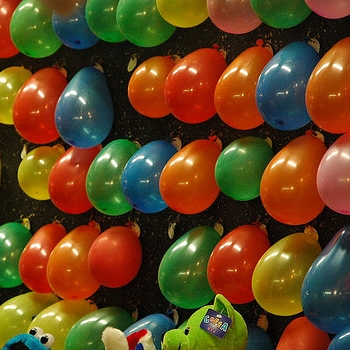
\includegraphics[width=\textwidth]{images/balloons/balloons-original.jpg}
        \caption{Balloons, RGB color image \cite{balloons}.}
        \label{fig:balloons-rgb}
    \end{minipage}
    \hspace{0.5cm}
    \begin{minipage}[t]{0.45\linewidth}
        \centering
        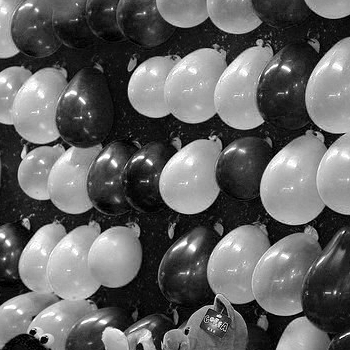
\includegraphics[width=\textwidth]{images/balloons/balloons-red-channel.jpg}
        \caption{Balloons, red channel \cite{balloons}.}
        \label{fig:balloons-red}
    \end{minipage}
\end{figure}
\begin{figure}[ht]
    \begin{minipage}[t]{0.45\linewidth}
        \centering
        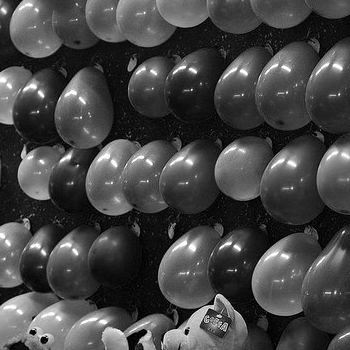
\includegraphics[width=\textwidth]{images/balloons/balloons-green-channel.jpg}
        \caption{Balloons, green channel \cite{balloons}.}
        \label{fig:balloons-green}
    \end{minipage}
    \hspace{0.5cm}
    \begin{minipage}[t]{0.45\linewidth}
        \centering
        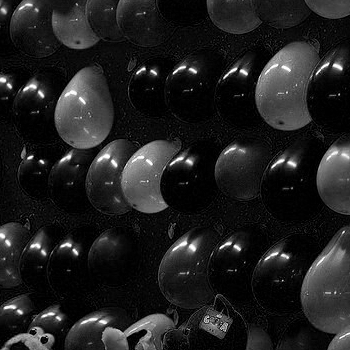
\includegraphics[width=\textwidth]{images/balloons/balloons-blue-channel.jpg}
        \caption{Balloons, blue channel \cite{balloons}.}
        \label{fig:balloons-blue}
    \end{minipage}
\end{figure}

An example to this can be seen in figures \ref{fig:balloons-rgb},
\ref{fig:balloons-red}, \ref{fig:balloons-green} and \ref{fig:balloons-blue}.
Figure \ref{fig:balloons-rgb} is the original in RGB color. Figure \ref{fig:balloons-red},
\ref{fig:balloons-green} and \ref{fig:balloons-blue} represent the intensity in the red,
green and blue channel respectively. A region in an image that is white (high
intensity) in all three channels is white in the RGB original as well, this can
be seen in the lower left as the eyeballs of the cuddly toy. A region that is white
in red channel and black in the blue and green channel is red in the RGB original, as
can be seen for all red balloons.

Though looking at only two channels can not tell the entire truth. As an example all
yellow balloons could be interpreted as red ballons if you only look at the
red and blue channels. The only difference between red and yellow balloons is
seen in the green channel where the intensity of yellow balloons is higher than
there red counterparts.

The RGB color space is one of the standard color models used today, other models
worth mentioning is the CMY (or CMYK) and HSI color model. These color space
models are out of scope of this report. For more information about them,
reading chapter 6 of "Digital image processing" by Gonzalez and Woods \cite{gonzalez2008} is suggested.

As an image always is two dimensional it's common to describe its intensity as
a function of x and y coordinates (Eq. \ref{eq:intensity}). The indexing of
rows and columns starts in the upper left corner with element (0,0) and increases
in x direction downwards and in y direction to the right. As an example if an
image has 100 pixels in a square the bottom right pixel will be indexed (10,10) \cite[p. 56]{gonzalez2008}.
\begin{equation}
    \label{eq:intensity}
    I(x,y)
\end{equation}

\subsection{Filtering and Gaussian smoothing}
An image's quality depends on a lot of factors. During aquisition some kind of
camera is used, first of all the quality of the image depends on the quality
of the camera. The lens and sensor needs to be adequate for its usage.
It also depends on how the image is stored, many mobile phone cameras store
the images in compressed format and there is no way to get the uncompressed
image back. Independent of how an image is aquired the image will always have
some artifacts, or in another term, some noise in it. This noise can be described
as a part of the image that is displayed on a computer. From equation \ref{eq:intensity}
 the true intensity from a pixel is given and the noise is added to it as \(n(x,y)\) in
 equation \ref{eq:intensityNoise}, the result is the image as it's displayed. In other
 terms the image that you view on a computer is never perfect, it always has some
 noise or artifacts in it \cite[p. 76]{gonzalez2008}.
\begin{equation}
    \label{eq:intensityNoise}
    \hat{I}(x,y) = I(x,y) + n(x,y)
\end{equation}

The problem to remove as much noise as possible but still keep key features of
an image, is a big problem. The reason for this is that noise can be described
as a high variation in intensity between neighbouring pixels and the exact
same description can be used for describing edges between different regions
in an image. To solve this problem some help is gathered from the field of
statistics. Noise is unknown for each pixel otherwise it wouldn't be noise.
From the field of statistics the concept of distribution can be
useful. If the noise is modeled as some distribution it could to some extent
be reversed to give a much better finished image. This is what the
gaussion distribution and gaussion filter is about. Gaussion distribution in 1
dimension is defined in equation \ref{eq:gaussianDistribution1D}, \cite[p. 314]{gonzalez2008}.
\begin{equation}
    \label{eq:gaussianDistribution1D}
    P(x) = \frac{1}{{\sigma \sqrt {2\pi } }}e^{{{ - \left( {x - \bar{x}} \right)^2 } \mathord{\left/ {\vphantom {{ - \left( {x - \mu } \right)^2 } {2\sigma ^2 }}} \right. \kern-\nulldelimiterspace} {2\sigma ^2 }}}
\end{equation}
\begin{equation}
    \label{eq:gaussianDistribution1DZeroMean}
    P(x) = \frac{1}{{\sigma \sqrt {2\pi } }}e^{-\frac{x^2}{2 \sigma^2}}
\end{equation}

In equation \ref{eq:gaussianDistribution1D}, x is the intensity of a pixel, \(\bar{x}\)
is the mean value of x and \(\sigma\) is its standard deviation. With a zero mean
(function centered around 0) equation \ref{eq:gaussianDistribution1DZeroMean} is the result.
The distribution takes the form of a bell curve and a few examples can be seen in figure
\ref{fig:gaussian1d}.
\begin{figure}[ht]
    \begin{minipage}[t]{\linewidth}
        \centering
        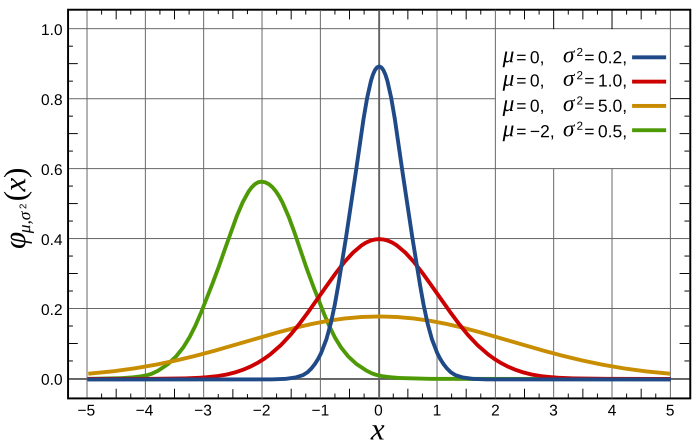
\includegraphics[width=\textwidth]{images/gaussian1d.png}
        \caption{Different values for the Gaussian distribution. \(\mu\) is the mean and \(\sigma\) is the standard deviation. Image from Wikipedia \cite{wiki:distributionGraph}.}
        \label{fig:gaussian1d}
    \end{minipage}
\end{figure}
As images have 2 dimensions the equation needs to be for that. Gaussion distribution in 2
dimensions have the form that can be seen in equation \ref{eq:gaussianDistribution2D}.
\begin{equation}
    \label{eq:gaussianDistribution2D}
    P(x,y) = \frac{1}{{ 2\pi \sigma^2}}e^{- \frac{x^2 + y^2}{2 \sigma^2}}
\end{equation}
To visualise the distribution in 2 dimensions one could think of a hill with even
slopes all around the center. Depending on input values such as the mean and
standard deviation the hill gets different shapes. With higher sigma the
hill will be lower and the sides will be flatter.

The next issue to deal with is that the function is continous but images are
structured in discrete rows and columns, there is no pixel at position \(x=1.5\) only
at \(x=1\) and \(x=2\). So to be able to do a Gaussian smoothing on an image a
discrete approximation of equation \ref{eq:gaussianDistribution2D} needs to be made.
The approximation is structured in an odd numbered matrix e.g. 3x3 or 5x5, this
is what is called the kernel or mask when it comes to image filtering.

% TODO: Add information about how to use the kernel
How to apply this kernel to smooth an image is out of scope for this report.
To learn more about this suggested reading is Digital Image Processing chapter 3.4
{\em Fundamentals of Spatial Filtering} \cite{gonzalez2008} or
watch the lecture about this topic by Dr. Mubarak Shah \cite{youtube:lectureFiltering}.

% 0. The purpose to remove artifacts.
% 1. Start with statistics normal distribution and standard deviation.
% 2. Continue with one dimensional example.
% 3. Move to 2 dimensional
% 4. Introduce the kernel and apply it to some image (smile)

\subsection{Image segmentation}
A big part of digital image processing is taking an image, modify it and
return a new image. Image segmentation is instead taking an image as input,
identifying interesting regions and return thoose regions back to the user.
This could be done for detecting veins and arteries in medical images \cite{olena2010},
for detecting objects moving across a road or identifying missing components on
a circuit board in a factory during the certification process in the end of a production line.
Image segmentation is a main step before object recognition can be made.

The most basic image segmentation methods try to identify points, lines and edges
and work from there.

% TODO: Can add mathematical details about isolated point detection.

\section{The algorithm}
This section will go through the Efficient Graph-Based Image Segmentation
algorithm introduced by Pedro F. Felzenswalb and Daniel P. Huttenlocher \cite{felzenszwalb2004}.
To help the explanation throughout the chapter four images will be used, that is figure \ref{fig:smile-rgb},
\ref{fig:smile-red}, \ref{fig:smile-green} and \ref{fig:smile-blue}.

The algorithm is constructed in a general fashion which makes it possible to use
under many different settings. The key parts needed are an undirected graph and
some weight on each edge in the graph. As an example to this figure \ref{fig:smile-red}
can help, the red channel from the "smile" image. The image is 10x10 pixels in
size and construction of the undirected weighted graph is done by comparing
neighbouring pixels with each other. All pixels except the ones around the border
are connected to 8 neighbours (right,left,up,down and all four corners).
In other words the connectivity is chosen to be 8. Other types of connectevity
is 4-adjacency or mixed adjacency.

% TODO: Short example with image about connectivity?

When building the graph each edge get a weight that is the difference between
intensity in connected pixels. Pixel \(I(0,0)\) is mostly black so a good estimate
is that it has an intensity level of 10. The neighbour to the right \(I(0,1)\) has
the same intensity but the two neighbours downwards \(I(1,0)\) and \(I(1,1)\) are
white. An estimate for the white color is 250 in intensity. The edge weight is
now calculated to 0 between the two black pixels and 240 between the black and the
two white pixels.

\begin{figure}[ht]
    \begin{minipage}[t]{0.45\linewidth}
        \centering
        
\includegraphics[width=\textwidth]{images/smile/smile-original.jpg}
        \caption{Smile, RGB color image}
        \label{fig:smile-rgb}
    \end{minipage}
    \hspace{0.5cm}
    \begin{minipage}[t]{0.45\linewidth}
        \centering
        
\includegraphics[width=\textwidth]{images/smile/smile-red-channel.jpg}
        \caption{Smile, red channel.}
        \label{fig:smile-red}
    \end{minipage}
\end{figure}
\begin{figure}[ht]
    \begin{minipage}[t]{0.45\linewidth}
        \centering
        
\includegraphics[width=\textwidth]{images/smile/smile-green-channel.jpg}
        \caption{Smile, green channel.}
        \label{fig:smile-green}
    \end{minipage}
    \hspace{0.5cm}
    \begin{minipage}[t]{0.45\linewidth}
        \centering
        
\includegraphics[width=\textwidth]{images/smile/smile-blue-channel.jpg}
        \caption{Smile, blue channel.}
        \label{fig:smile-blue}
    \end{minipage}
\end{figure}

With the undirected weighted graph built it's time to take a closer look at the
segmentation. The goal with the algorithm is to be fast and {\em "Capture perceptually
important groupings or regions, which often reflect global aspects of the image"} \cite{felzenszwalb2004}.
One easy way to segment an image is to say that all edges that are less than some
constant \(k\) should belong to the same region. So in the example image, figure \ref{fig:smile-red},
it would work pretty well as all the regions that are visually considered to belong
together would be grouped together. The problem arises as soon as this is tried
on a "real" image that has not been created on a computer. Remember the discussion
about noise from earlier chapter. Noise in just one pixel, e.g. the center
pixel in one of the eyes could cause the algorithm (with constant \(k\)) to divide
the eye into 5 different regions.

Instead of a constant that decides whether a pixel should belong to a region or
not Felzenswalb and Huttenlocher have come up with a predicate that is variable
and takes the neighbouring regions into account. To continue explaining the
algorithm some terminology and a more mathematical approach is needed. The following
paragraphs until the end of this chapter are the key parts from the original paper \cite[ch. 3.1 Pairwise
Region Comparison Predicate]{felzenszwalb2004}.

The goal is to decide whether there should be a boundary between two pixels or
two pixels should belong to the same component. A component is a connected region of one
or more pixels. Let \(D\) be the predicate that is true if there should be a
boundary or false if the two pixels should belong to the same component. Before
defining \(D\) two other definitions are needed. First of all the definition
of {\em internal difference}.
\begin{equation}
    \label{eq:internalDifference}
    \text{Int}(C) = \underset{e \in \text{MST}(C,E)}{\text{max}} w(e)
\end{equation}

\(Int(C)\), the internal difference in a component is the maximum weight of
all edges within that component. As an example if four pixels, that belongs to the same component,
are connected with the edge weights 50, 100 and 150. The internal difference
would be 150. Next up is the {\em difference between} components.
\begin{equation}
    \label{eq:differenceBetween}
    \text{Dif}(C_1,C_2) = \underset{v_i \in C_1,v_j \in C_2, (v_i,v_j) \in E}{\text{min}} w((v_i,v_j))
\end{equation}
The difference between two components is the minimum weight edge between the
components. With the internal difference and the difference between two components,
it's time to define the predicate.
\begin{equation}
    \label{eq:predicate}
    D(C_1,C_2) =
    \begin{cases}
        true & \text{if } Dif(C_1,C_2) > MInt(C_1,C_2) \\
        false & otherwise
    \end{cases}
\end{equation}
The predicate says that there is reason for a border (true) if the difference
between two components is larger than the minimum internal difference, \(MInt\),
in the two components. In equation \ref{eq:internalDifference} the internal
difference is defined for one component though with that definition the predicate
in equation \ref{eq:predicate} is not very good for small components. So instead
of just selecting the minimum internal difference in components a threshold function
is added.
\begin{equation}
    \label{eq:minimumInternal}
    \text{MInt}(C_1,C_2) = \text{min}(\text{Int}(C_1) + \tau(C_1),\text{Int}(C_2) + \tau(C_2))
\end{equation}
\begin{equation}
    \label{eq:threshold}
    \tau(C) = \frac{k}{|C|}
\end{equation}
The threshold function will depend on the size of the components being compared
and will be most important for small components and as the components grove the
weight of the threshold function will fade away. This finishes of the definition
of the predicate and it's time to look at the actual steps taken in the
algorithm.

The efficient graph-based image segmentation algorithm takes a graph as input
\(G = (V,E)\) with \(n\) vertices and \(m\) edges. Remember from earlier chapter
that in image segmentation it's not a new image that is the output instead it's
the regions that have been found in the image. The output in the following text
is defined as \(S = (C_1,...,C_r)\). The algorithm has five main steps and the
steps are as follows.
\begin{enumerate}
    \item Sort all edges \(E\) in non-decreasing order.
    \item All pixels are their own component from start.
    \item Repeat step 4 for all edges.
    \item Select the edge with the lowest weight and use the predicate defined in
        equation \ref{eq:predicate} to decide whether the components should belong
        to the same component or leave them in separate components. Merge components
        if needed.
    \item Return S with all components.
\end{enumerate}
\subsection{Pros and cons}
The algorithm is versatile and fast, as long as you have a weighted undirected graph
it will work, depending on application the results will vary. An example to this
are the figures \ref{fig:smile-rgb} to \ref{fig:smile-blue}. You could either
run the algorithm directly on a graph with weights built from the RGB value or
you can build three different graphs, one for each channel and run the
algorithm three times and merge thoose components that are found to be
components in each channel. 

Felzenszwalb and Huttenlocher \cite{felzenszwalb2004} writes that the threshold
function can be changed as long as it's a non-negative function. It can be
adapted to different shapes. {\em Such a shape preference could be as weak as
    preferring components that are not long and thin (e.g., using a ratio
of perimeter to area) [...]} \cite{felzenszwalb2004}. This shows how versatile
the algorithm is.

For a more detailed explanation of the algorithm and its pros and cons the
original paper which introduced the algorithm is listed in the references as \cite{felzenszwalb2004}.

% TODO: Add basics about Kruskal's minimum spanning tree.

% TODO: Add detailed gaussion description in digital image processing and
% then describe the difference here what it means to increase sigma value.

% TODO: Show an simple color image that has some differences when it
% comes to 4 or 8 connectness.

% \subsection{Building the graph}
% \subsection{Threshold function}
% What about taking into account width and breadth but crossings wouldn't
% count and curved roads would not be found.

\section{Application}
The main goal from the start has been to identify roads from Bing aerial maps.
To try this out an account with Bing maps API has been set up for educational
purposes. Two different locations were chosen as example areas to try the algorithm
on. The implementation used is the one created by Felzenszwalb and found on
his webpage at Brown University homepage \cite{web:sourceCode}. The additions
made to the algorithm is a wrapper with OpenCV library \cite{web:wrapper}.
The additions the wrapper gives is a GUI for faster testing of different
input values and the possibility to load any image type supported by OpenCV.

The first location is an aerial image over central parts of Lule\.{a} in northern
Sweden. The original is shown in figure \ref{fig:luleaOriginal} and the segmentation
is shown in figure \ref{fig:luleaEGBIS}.
\begin{figure}[ht]
    \begin{minipage}[t]{\linewidth}
        \centering
        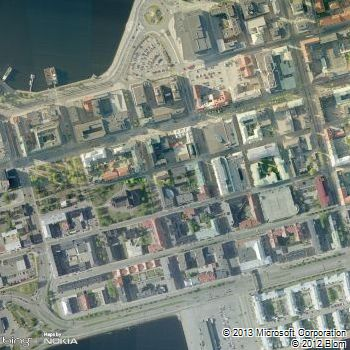
\includegraphics[width=\textwidth]{images/bing/lulea-original.jpg}
        \caption{Lule\.{a}, image from Bing Maps API}
        \label{fig:luleaOriginal}
    \end{minipage}
\end{figure}
The result from this segmentation presented here is one of the best. With other
values for input the segmentation becomes either to detailed or too rough
(too big regions).
\begin{figure}[ht]
    \begin{minipage}[t]{\linewidth}
        \centering
        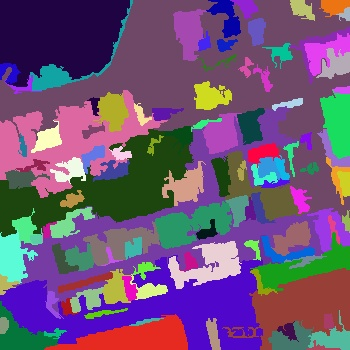
\includegraphics[width=\textwidth]{images/bing/lulea-egbis.jpg}
        \caption{Lule\.{a}, EGBIS segmentation, sigma at 0.8, k at 300 and c at 100}
        \label{fig:luleaEGBIS}
    \end{minipage}
\end{figure}

In figure \ref{fig:roadOriginal} a region with mostly forest, one highway passing
through in the middle and a few roads connecting to the highway at a junction is shown.
The segmentation from this is shown in \ref{fig:roadEGBIS}. The result shows
the highway clearly in the middle as a region but the smaller roads and the junction
is hard to identify unless you know that they exist.
\begin{figure}[ht]
    \begin{minipage}[t]{\linewidth}
        \centering
        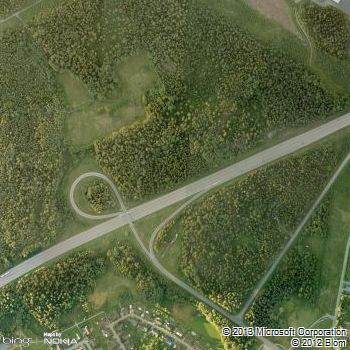
\includegraphics[width=\textwidth]{images/bing/road-original.jpg}
        \caption{Highway, image from Bing Maps API}
        \label{fig:roadOriginal}
    \end{minipage}
\end{figure}
\begin{figure}[ht]
    \begin{minipage}[t]{\linewidth}
        \centering
        
\includegraphics[width=\textwidth]{images/bing/road-egbis.jpg}
        \caption{Highway, EGBIS segmentation, sigma at 0.8, k at 300 and c at 100}
        \label{fig:roadEGBIS}
    \end{minipage}
\end{figure}

\section{Conclusions}
A big problem within the field of image segmentation is to define and judge
what a good segmentation is. If an algorithm identifies one part of an image
in the foreground while another identfies something else in the background, which
one is better is hard to say. What can be said is when the result is not adequate
for post processing such as road recognition in this case.

The image over Lule\.{a} clearly shows some roads while other parts of the
image are more vague even for the human eye. The segmentation gives some hints
to what could be roads but the detail is not enough for future work to be worth it.
The second image which basically is a highway with a junction through a forest
should be relatively easy to segment. Segmentation of the highway image shows
the road going through the central parts of the image and can be defined as
a good segmentation if it's only the highway that is to be identified. The smaller
roads are near impossible to see in the segmentation.

The two images tested in this case shows that the Efficient Graph-Based Image Segmentation
is not viable for this application. There may be future work that can be done
to create a better threshold function to detect thinner lines.

This project started out with the algorithm and application, the result as stated
above is not satisfactory so future work should start with more specific algorithms
for road recognition. Example of work that can be intresting to look closer to
is listed below.
\begin{itemize}
  \item {\em "Automatic Road Extraction from Aerial Images"} by John C. Trinder and
Yandong Wang \cite{trinder1998}.
  \item {\em "Detection of Roads in Aerial Images by
Using Edge Information"} by Wu-Ja Lin and Chih-Wei Tseng \cite{lin2012}.
  \item {\em "Urban Road Extraction from High-Resolution Optical Satellite Images"} by
Mohamed Naouai, Atef Hamouda and Christiane Weber \cite{naouai2010}.
  \item {\em "Unsupervised line network extraction in remote sensing using a polyline
      process"} by Caroline Lacoste, Xavier Descombes and Josiane Zerubia \cite{lacoste2009}.
\end{itemize}

% The eye sees some different shapes that is not there we make them up in our
% mind.
% \nocite{*}

%\end{document}  % This is where a 'short' article might terminate

% Just comment this out if we don't need it.
%\input{acknowledgment.tex}

%
% The following two commands are all you need in the
% initial runs of your .tex file to
% produce the bibliography for the citations in your paper.
\bibliographystyle{abbrv}
\bibliography{sigproc}  % sigproc.bib is the name of the Bibliography in this case
% You must have a proper ".bib" file
%  and remember to run:
% latex bibtex latex latex
% to resolve all references
%
% ACM needs 'a single self-contained file'!
%
%APPENDICES are optional
%\balancecolumns
%\appendix
%Appendix A
%\section{Headings in Appendices}
%The rules about hierarchical headings discussed above for
%the body of the article are different in the appendices.
%In the \textbf{appendix} environment, the command
%\textbf{section} is used to
%indicate the start of each Appendix, with alphabetic order
%designation (i.e. the first is A, the second B, etc.) and
%%a title (if you include one).  So, if you need
%hierarchical structure
%\textit{within} an Appendix, start with \textbf{subsection} as the
%highest level. Here is an outline of the body of this
%document in Appendix-appropriate form:
%\subsection{Introduction}
%\subsection{The Body of the Paper}
%\subsubsection{Type Changes and  Special Characters}
%\subsubsection{Math Equations}
%\paragraph{Inline (In-text) Equations}
%\paragraph{Display Equations}
%\subsubsection{Citations}
%\subsubsection{Tables}
%\subsubsection{Figures}
%\subsubsection{Theorem-like Constructs}
%\subsubsection*{A Caveat for the \TeX\ Expert}
%\subsection{Conclusions}
%\subsection{Acknowledgments}
%\subsection{Additional Authors}
%This section is inserted by \LaTeX; you do not insert it.
%You just add the names and information in the
%\texttt{{\char'134}additionalauthors} command at the start
%of the document.
%\subsection{References}
%Generated by bibtex from your ~.bib file.  Run latex,
%then bibtex, then latex twice (to resolve references)
%to create the ~.bbl file.  Insert that ~.bbl file into
%the .tex source file and comment out
%the command \texttt{{\char'134}thebibliography}.
% This next section command marks the start of
% Appendix B, and does not continue the present hierarchy
%\section{More Help for the Hardy}
%The acm\_proc\_article-sp document class file itself is chock-full of succinct
%and helpful comments.  If you consider yourself a moderately
%experienced to expert user of \LaTeX, you may find reading
%it useful but please remember not to change it.
\balancecolumns
% That's all folks!
\end{document}
